%! Author = Vojta
%! Date = 21.1.2024

\chapter{Technologie}
\label{chap:technologie}

\section{Úvod}
Tato kapitola poskytuje podrobný přehled a analýzu technologií použitých v rámci diplomové práce. Správný výběr technologických nástrojů je zásadní nejen pro funkčnost a efektivitu finálního produktu, ale také ovlivňuje proces vývoje, údržbu a možnosti dalšího rozvoje projektu. Základem projektu jsou moderní technologie a \emph{frameworky}, které jsou velmi populární v oblasti webového vývoje. Mezi klíčové technologie patří frontendový \emph{framework} Vue společně s \emph{metaframeworkem} Nuxt, jazyk TypeScript a Tailwind pro stylování. Každá z těchto technologií byla vybrána na základě zkušeností autora, potřeb projektu a jejich schopnosti efektivně adresovat požadavky na vývojářskou a uživatelskou přívětivost. Následující sekce poskytne rozbor důvodů vedoucích k výběru těchto nástrojů a popis, jak jednotlivé technologie spolupracují na dosažení stanovených cílů.

\section{Dokumentace a komponenty}
Tato sekce se věnuje technologiím a nástrojům, které budou použity pro dokumentaci a vývoj komponent.

\subsection{Vue}
Vue.js je \emph{framework} pro JavaScript zaměřený na tvorbu uživatelských rozhraní. Vychází z běžných webových technologií, jako jsou HTML, CSS a JavaScript, a přináší model programování založený na komponentách a deklarativním přístupu, který usnadňuje vývoj rozhraní různých úrovní složitosti.

Dvě klíčové funkce Vue:

\begin{itemize}
  \item Deklarativní vykreslování: Vue rozšiřuje standardní HTML pomocí šablony syntaxe, která umožňuje deklarativně specifikovat výstup HTML založený na stavech v JavaScriptu.
  \item Reaktivita: Vue efektivně monitoruje změny ve stavech JavaScriptu a při těchto změnách automaticky a efektivně aktualizuje DOM. \cite{WhatIsVue}
\end{itemize}

Vue je známé svou jednoduchostí a flexibilitou, což z něj činí ideální volbu pro vývojáře různých úrovní zkušeností. V rámci této diplomové práce je Vue použito jako základní technologie pro tvorbu komponent. Avšak komponenty nemusí být 100\% kompatibilní s čistým Vue, protože se zde používají některé funkce, které jsou dostupné pouze v rámci \emph{frameworku} Nuxt.

\subsection{Nuxt}
Nuxt je moderní a výkonný open source \emph{framework} založený na Vue, který je navržen pro intuitivní a efektivní vývoj webových aplikací a stránek. Tento \emph{framework} se vyznačuje tím, že automaticky řeší mnoho opakujících se úkolů vývojářů, což jim umožňuje soustředit se na tvorbu samotné aplikace. Nuxt využívá konvence a strukturované adresářové uspořádání pro automatizaci procesu vývoje a nabízí možnost vlastní konfigurace a přizpůsobení výchozích chování.

Nuxt má narozdíl od čistého Vue schopnosti server-side renderingu (SSR). Tato funkce zajišťuje rychlejší načítání stránek a lepší SEO, protože celý obsah stránky je serverem vygenerován dříve, než začne běžet klientský JavaScript. Nuxt tento přístup kombinuje v takzvaném hybrid renderingu a má tedy výhody tradičního server-side renderingu s interaktivitou a pokročilými uživatelskými rozhraními single-page aplikací (SPA). \cite{NuxtRenderingModes}

\subsection{Tailwind}
Tailwind je moderní a oblíbený CSS \emph{framework} \cite{StateOfCSS} \cite{StateOfFrontend}, který se zaměřuje na tzv. \emph{utility-first} přístup. Tento přístup umožňuje vývojářům rychle a efektivně vytvářet vlastní komponenty a designy s použitím nízkoúrovňových CSS tříd, které jsou přímo integrovány do HTML markupu.

Jednou z hlavních výhod Tailwind je možnost psát méně vlastního CSS. Vývojáři mohou využívat předdefinované třídy, jako jsou \emph{flexbox} a padding utility, což znamená, že většina stylů je opakovaně použitelná a zřídka je potřeba psát nové CSS. Tailwind také eliminuje potřebu vymýšlet názvy tříd, protože vývojáři vybírají třídy z předdefinovaného designového systému. To znamená, že nemusí přemýšlet o \uv{dokonalých} názvech tříd pro určité styly a komponenty nebo si pamatovat složité názvy. \cite{TailwindUtilityFirst}

Tailwind je známý svou flexibilitou a kontrolou nad tím, jak aplikace vypadá, což poskytuje větší prostor pro vytváření jedinečných webů. Na rozdíl od jiných CSS \emph{frameworků}, jako je Bootstrap nebo Materialize, Tailwind nenabízí plně stylované komponenty, jako jsou tlačítka nebo \emph{dropdown} menu. Místo toho nabízí utility třídy, které umožňují vytvořit vlastní opakovaně použitelné komponenty.

Přestože Tailwind nabízí mnoho výhod, může být jeho použití obtížné pro ty, kteří nejsou zkušení s CSS, a může způsobovat zmatek kvůli množství informací uložených v HTML souboru. Navíc při instalaci Tailwindu jsou výchozí CSS styly resetovány \cite{TailwindPreflight}, takže je nutné je pro všechny elementy znovu vytvořit.

Tailwind bude v této diplomové práci použit pro stylování komponent a stránek. Také je využit pro tvorbu motivů a brandingu pomocí jeho konfiguračního souboru a CSS proměnných.

\subsection{TypeScript}
TypeScript je nadstavba jazyka JavaScript, která přidává statické typování a další pokročilé vlastnosti, jež zvyšují kvalitu a udržitelnost kódu ve velkých softwarových projektech. Díky kompatibilitě s JavaScriptem umožňuje TypeScript vývojářům využívat veškeré existující knihovny a \emph{frameworky}, zároveň ale poskytuje výhody striktnějšího typového systému, jako jsou například lepší nástroje pro refaktoring, snazší navigace v kódu a vyšší bezpečnost během kompilace. V diplomové práci je TypeScript využíván pro zlepšení spolehlivosti aplikace a minimalizaci chyb za běhu, což je zvláště důležité při vývoji komplexních systémů s mnoha interakcemi mezi komponenty. Přidání typů do kódu umožňuje vytvářet lepší dokumentaci a zlepšit komunikaci mezi členy vývojového týmu, což zjednodušuje rozvoj a údržbu projektu. V kombinaci s \emph{frameworkem} Vue a Nuxt, TypeScript přináší výrazné vylepšení v rychlosti vývoje a kvalitě výsledného produktu. \cite{TypeScript}

% Porovnání TS vs. JS a proč v tomto projektu dává smysl použít TS

\subsection{Nuxt Content}
Nuxt Content je \emph{headless} CMS založený na verzovacím systému Git pro Vue vývojáře. Umožňuje vytvářet obsah pomocí Markdown a JSON a dotazovat se na něj pomocí API podobného MongoDB. \cite{NuxtContent}

Nuxt Content je modul pro \emph{framework} Nuxt, který usnadňuje práci s obsahem. Tento modul umožňuje vývojářům psát obsah přímo v Markdown, YAML, JSON, a XML souborech a efektivně je integrovat do Nuxt aplikací. Obsah je možné snadno načítat a zobrazovat díky jednoduchému API, které Nuxt Content nabízí. Kromě snadného načítání dat, modul poskytuje nástroje pro full-textové vyhledávání, což je velmi užitečné dokumentace, blogy a další aplikace, které vyžadují efektivní správu obsahu. Integrace s Vue komponentami je přímá a bezproblémová, což výrazně zlepšuje workflow vývojářů a umožňuje jim věnovat více času na kreativní aspekty projektu, místo zbytečného řešení technických detailů správy obsahu.

V této diplomové práci bude Nuxt Content využit pro dokumentaci komponent a strukturovaný obsah, který je snadno editovatelný a spravovatelný v rámci Git repozitáře. Nuxt Content je ideální volbou, protože nevyžaduje žádnou další infrastrukturu.

\subsection{Shiki}
Shiki je knihovna pro syntax highlighting, která je založena na stejném mechanismu, jaký používá Visual Studio Code. Tato technologie poskytuje vysoce přesné a vizuálně atraktivní zvýrazňování syntaxe pro širokou škálu programovacích jazyků. Shiki umožňuje snadnou integraci do různých webových projektů díky svému API a podporuje načítání různých barevných témat, což umožňuje vývojářům přizpůsobit vzhled zvýraznění kódu svým specifickým potřebám. Efektivita a flexibilita Shiki v integraci a konfiguraci z něj činí ideální nástroj pro projekty, které vyžadují zobrazení zdrojového kódu v dokumentaci nebo výukových materiálech, přičemž zachovává konzistenci a čitelnost prezentovaného kódu. \cite{Shiki}

V této diplomové práci bude Shiki použit pro zvýrazňování syntaxe v dokumentaci a ukázkových kódech, což zvyšuje čitelnost obsahu a usnadňuje vývojářům rychleji porozumět kódu.

\begin{figure}[H]
  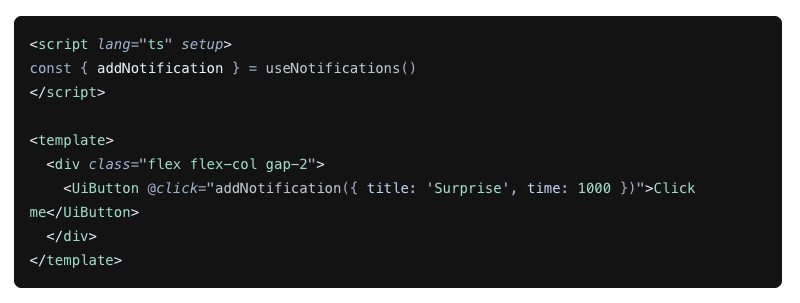
\includegraphics[width=\textwidth]{images/shiki}
  \caption{Zvýraznění kódu pomocí Shiki} \label{picture:shiki}
\end{figure}

\subsection{Headless UI}
Nestylované, přístupné UI komponenty, navržené tak, aby se jednoduše používaly s Tailwind CSS. \cite{HeadlessUI}

Headless UI je sada přístupných UI komponent, které jsou navrženy tak, aby byly snadno integrovatelné do jakéhokoliv designu nebo frontendového \emph{frameworku}. Tato knihovna poskytuje základní funkční strukturu pro běžné UI prvky, jako jsou rozbalovací menu, přepínače a dialogová okna, ale neobsahuje žádné vlastní styly, což umožňuje vývojářům plně ovládat vzhled těchto komponent. Headless UI je ideální pro projekty, které vyžadují vysokou míru přizpůsobení a chtějí používat specifický designový jazyk bez nutnosti bojovat s předdefinovanými styly. Komponenty jsou navrženy s ohledem na přístupnost, což zajišťuje, že aplikace jsou použitelné pro širokou škálu uživatelů, včetně těch s omezenými schopnostmi. Headless UI tak usnadňuje vytváření robustních a esteticky příjemných webových aplikací, které jsou zároveň přístupné a uživatelsky přívětivé.

V této diplomové práci bude Headless UI použito pro tvorbu základních UI komponent, jako jsou modální okna, navigační lišty či další prvky. Tato knihovna poskytuje flexibilitu a kontrolu nad vzhledem komponent, což je důležité pro jednoduché úpravy a rozšíření.

\subsection{Floating UI}
Floating UI je JavaScriptová knihovna navržená pro pozicování plovoucích prvků, jako jsou \emph{tooltipy}, \emph{popovery} a \emph{dropdown} menu, a umožňuje také vytváření interakcí pro tyto prvky. Knihovna se zaměřuje na robustní ukotvení absolutně pozicovaných plovoucích prvků vedle referenčních prvků s funkcemi, které zabraňují kolizím s okrajem zobrazení, čímž zajišťuje, že plovoucí prvky zůstanou vždy viditelné a optimálně umístěné.

Floating UI podporuje různé platformy včetně webu, React, React Native a Vue, a je vysoce modulární, což umožňuje vývojářům použít jen tolik funkcionality, kolik potřebují, což může vést k optimalizaci velikosti balíčku. Dále je knihovna navržena tak, aby byla flexibilní a umožňovala snadnou integraci bez omezení na specifické technologie nebo \emph{frameworky}. \cite{FloatingUI}

V této diplomové práci bude Floating UI použito pro tvorbu interaktivních prvků, jako jsou \emph{tooltipy} a \emph{popovery}, které zvyšují uživatelskou interaktivitu a zlepšují uživatelskou zkušenost. Důležité je především zabránění přetékání prvků mimo obrazovku a zajištění, že plovoucí prvky jsou vždy viditelné a snadno přístupné.

\subsection{Embla Carousel}
Embla Carousel je malá, open source knihovna pro JavaScript, která se zaměřuje na tvorbu pohyblivých prvků, jako jsou \emph{carousely}, s vysokou přesností pohybu a skvělou reakcí na gesta. Tato knihovna je navržena tak, aby byla nezávislá na jiných knihovnách a nevyžaduje žádné další závislosti. \cite{EmblaCarousel}

Embla Carousel nabízí možnost snadné integrace do různých \emph{frameworků} jako React, Vue, Svelte a Solid, díky čemuž je flexibilní pro různé typy projektů. Využívá moderní CSS vlastnosti, jako je \emph{flexbox}, pro definování velikosti a mezer mezi prvky a podporuje i pokročilé funkce, jako je automatické přehrávání a responzivní nastavení.

K dispozici jsou různé pluginy, které rozšiřují základní funkčnost, včetně možností pro automatické přehrávání, \emph{auto-scroll}, a adaptaci výšky. Embla také poskytuje rozsáhlé API pro pokročilé manipulace a přizpůsobení \emph{carouselů}, což umožňuje vývojářům plně ovládat chování a vzhled \emph{carouselů} podle potřeb projektu.

V této práci bude Embla Carousel použit pro tvorbu \emph{carousel} komponenty. Díky vysoké flexibilitě poskytuje nepřeberné možnosti konfigurace a přizpůsobení.

\section{CLI}
Tato sekce se věnuje technologiím a nástrojům, které byly použity pro vývoj CLI pro instalaci komponent.

\subsection{Commander.js}
Commander.js je oblíbená knihovna pro Node.js, která usnadňuje vytváření příkazových řádkových rozhraní (CLI). Umožňuje vývojářům definovat příkazy, volby a parametry pro jejich aplikace v jednoduchém a strukturovaném formátu. Commander.js poskytuje funkce, jako je automatické generování nápovědy, parsování příkazů a argumentů, a podporu pro subpříkazy, což umožňuje vývojářům snadno rozšiřovat funkčnost svých aplikací bez nutnosti psát rozsáhlý kód pro zpracování vstupů. Díky své flexibilitě a jednoduchosti použití se Commander.js stal standardním nástrojem pro mnoho projektů založených na Node.js. \cite{CommanderJS}

V této diplomové práci bude Commander.js použit pro vytvoření CLI pro instalaci komponent.

Jako alternativa se nabízí Citty z ekosystému UnJS. Má podobné funkce jako Commander, avšak v době tvorby této práce byla tato knihovna v rané fázi vývoje a nebyla dostatečně stabilní pro použití v produkčním prostředí. \cite{Citty}

\subsection{Ora}
Ora je minimalistická a efektivní knihovna pro Node.js, která umožňuje vývojářům přidat elegantní indikátory načítání (tzv. spinners) do jejich CLI. Tyto indikátory jsou užitečné pro zobrazování stavu dlouhotrvajících operací, aniž by uživatele zatěžovaly nadměrnými informacemi. Ora nabízí širokou škálu přednastavených stylů a umožňuje také snadnou personalizaci, včetně změny textu, barvy a symbolů spinneru. Tato knihovna je oblíbená pro svou snadnou integraci a schopnost výrazně zlepšit uživatelskou zkušenost CLI aplikací tím, že poskytuje okamžitou vizuální zpětnou vazbu během procesů, které mohou trvat několik sekund nebo i déle. \cite{Ora}

V této diplomové práci bude Ora použit pro zobrazení indikátorů načítání během procesů instalace komponent.

\subsection{Prompts}
Prompts je knihovna pro Node.js, která umožňuje vývojářům snadno vytvářet interaktivní CLI. S pomocí této knihovny je možné efektivně spravovat uživatelské vstupy pomocí různých typů dotazů, jako jsou text, heslo, potvrzení a výběr z možností. Prompts podporuje asynchronní logiku, umožňuje validaci vstupů a podmíněné zobrazení dotazů, což vývojářům poskytuje flexibilitu pro vytváření složitějších scénářů interakcí. Tato knihovna je oblíbená pro svou jednoduchost, moderní API a minimální závislosti, což ji činí ideální volbou pro projekty, kde je potřeba rychle a efektivně zpracovávat uživatelské vstupy. \cite{Prompts}

V této diplomové práci bude knihovna Prompts použita pro interaktivní získávání informací od uživatele během procesu instalace komponent.

\subsection{Execa}
Execa je moderní knihovna pro Node.js, která zjednodušuje práci s externími procesy a příkazy shellu. Tato knihovna je navržena tak, aby vylepšila standardní Node.js metodu child\_process a poskytla lepší zkušenost s pokročilými funkcemi, jako je podpora asynchronních operací, vylepšená oblast viditelnosti výstupů procesů a lepší manipulace s chybami. Execa umožňuje snadné spouštění shell příkazů a jejich sledování v reálném čase, což je zvláště užitečné v automatizovaných skriptech a nástrojích pro vývoj. Díky execa lze také snadno získat textový výstup příkazů, což umožňuje vývojářům efektivně zpracovávat data bez nutnosti manuálního parsingu. \cite{Execa}

V této diplomové práci bude knihovna Execa použita pro instalaci závislostí během instalace komponent.

\subsection{Zod}
Zod je knihovna pro TypeScript, která slouží k vytváření schémat a validaci dat s cílem zajistit správnost typů během kompilace i za běhu. Zod umožňuje vývojářům definovat strukturu dat pomocí silného typového systému TypesSriptu, což vede ke snížení chyb způsobených neplatnými daty. Jednou z klíčových výhod Zodu je, že integrované validace se automaticky odrážejí ve vygenerovaných typech, což znamená, že jakékoli data splňující validaci jsou automaticky správně typována. Tato knihovna také podporuje složitější validační struktury, včetně vnořených objektů, pole, volitelných polí a unie typů, což ji činí ideálním řešením pro aplikace, které vyžadují přísnou kontrolu vstupních dat. \cite{Zod}

V této diplomové práci bude knihovna Zod použita pro definici schémat a validaci dat během procesu instalace komponent.

\subsection{Tsup}
Tsup je minimalistický a rychlý bundler pro TypeScript a JavaScript, postavený na technologii esbuild. Umožňuje vývojářům efektivně sestavovat své projekty s výrazným zlepšením v rychlosti sestavení oproti tradičním nástrojům jako je Webpack nebo Rollup. Tsup nabízí jednoduché CLI s několika konfiguračními možnostmi, což usnadňuje jeho používání a integraci do různých projektů. Mezi klíčové funkce patří podpora pro tree-shaking, generování deklarací TypeScript, a podpora pro ESM a CommonJS moduly. Díky své závislosti na esbuild, tsup poskytuje nejen rychlost, ale také efektivitu při minimalizaci a optimalizaci výsledného kódu.  \cite{Tsup}

V této diplomové práci bude tsup použit pro sestavení výsledného balíčku CLI pro instalaci komponent.

\section{Infrastruktura}
Tato sekce se věnuje technologiím a nástrojům, které byly použity pro správu kódu a jeho následné nasazení.

\subsection{pnpm workspaces}
pnpm workspaces jsou součástí správce balíčků pnpm, které umožňují efektivní správu více balíčků v rámci jednoho repozitáře (monorepo). Tato funkcionalita usnadňuje sdílení závislostí mezi projekty, což minimalizuje redundanci a zvyšuje efektivitu správy kódu. Workspaces podporují spojení více projektů pod jednou střechou s jednotnou správou závislostí, což je ideální pro velké projekty s mnoha podprojekty nebo knihovnami. Díky pnpm workspaces lze jednoduše instalovat závislosti pro všechny workspaces najednou, zatímco se zachovává úspora místa na disku a rychlost díky strategii pnpm pro sdílení závislostí. \cite{PnpmWorkspaces}

V této diplomové práci budou pnpm workspaces použity pro efektivní správu kódu v rámci monorepozitáře. Díky tomu, že jsou oba projekty (CLI a dokumentace) součástí jednoho repozitáře, je možné jednoduše testovat jejich propojení bez nutnosti stahování více repozitářů a jejich propojování, což zjednodušuje vývoj a údržbu.


\subsection{Changesets}
Changesets je nástroj, který pomáhá spravovat, verzovat a zveřejňovat změny v projektech s mnoha balíčky, typicky v monorepozitářích. Tento systém umožňuje vývojářům přidávat \uv{changeset}~soubory do git repozitáře, které popisují změny v balíčcích a jejich dopad na semantické verzování. Když přichází čas na vydání nové verze, Changesets automaticky generuje changelogy a aktualizuje verze balíčků podle pravidel semantického verzování. Tato metoda zajišťuje, že uživatelé knihovny mají jasné informace o tom, co každá verze zahrnuje. Changesets tak přináší transparentnost a předvídatelnost do procesu vývoje softwaru, což je zvláště cenné v prostředích, kde spolupracuje mnoho vývojářů. \cite{Changesets}

V této diplomové práci bude Changesets použit pro správu změn a verzování balíčků v rámci monorepozitáře. Tento nástroj zajišťuje, že všechny změny jsou správně dokumentovány a verzovány, což usnadňuje vydávání nových verzí.

\subsection{npm}
npm (Node Package Manager) je systém pro správu balíčků, který je standardně používán pro JavaScriptový runtime Node.js. npm umožňuje vývojářům snadno sdílet a spravovat závislosti kódu v jejich JavaScriptových projektech. Na oficiálních stránkách npm je dostupný obrovský repozitář obsahující přes 2,5 milionu balíčků, které může komunita využívat a přispívat do nich (v rámci open source repozitářů). Balíčky mohou obsahovat vše od malých knihoven až po komplexní \emph{frameworky}. \cite{Npm}

Přidání balíčku do npm je relativně jednoduchý proces, který začíná vytvořením účtu. Po přihlášení může vývojář vytvořit nový balíček pomocí příkazu npm init, který vede k nastavení balíčku včetně jeho názvu, verze, a závislostí. Po konfiguraci lze balíček publikovat na npm pomocí příkazu npm publish. Je důležité správně nastavit soubor package.json, který obsahuje metadata a závislosti balíčku. Vývojáři musí také zvážit licencování a další právní aspekty, aby byl jejich kód správně chráněn a licencován pro užití ostatními.

npx je nástroj přibalený s npm, který zjednodušuje spouštění balíčků nainstalovaných ve vašem Node.js prostředí nebo přímo z npm repozitáře bez nutnosti je explicitně instalovat. npx je užitečný zejména pro jednorázové spouštění balíčků nebo pro vyzkoušení nových nástrojů bez zatěžování vašeho lokálního vývojového prostředí. Když spustíte příkaz pomocí npx, například npx nuxi init my-app, npx automaticky stáhne potřebný balíček a jeho závislosti, spustí jej a po dokončení operace tyto dočasné instalace odstraní, čímž udržuje vaše prostředí čisté.

V této diplomové práci bude npm použito pro publikaci balíčku CLI pro instalaci komponent. Poté se pro jeho spuštění využívá npx.

\subsection{Github}
GitHub je jedna z největších a nejznámějších platforem pro správu softwarových projektů a verzování kódu pomocí systému Git. Umožňuje vývojářům hostovat a verzovat kód, spravovat projekty a sestavovat software společně s miliony dalších uživatelů po celém světě. GitHub poskytuje nástroje pro kolaborativní vývoj, jako jsou pull requesty (připojení nového kódu do dalších větví), správa větví a \emph{issues} pro každý projekt. Platforma se stala populárním nástrojem pro open source projekty, ale je rovněž populární mezi společnostmi pro soukromý vývoj softwaru díky svým robustním funkcím pro správu přístupu a integraci s různými externími službami. Dále, GitHub rozšiřuje své funkce o GitHub Actions, což jsou automatizační nástroje pro CI/CD procesy, které umožňují automatizovat testování a nasazování aplikací přímo z repozitářů na GitHubu. \cite{Github}

V této diplomové práci bude GitHub použit pro správu kódu a verzování projektu. Díky GitHub Actions jsou automatizovány procesy sestavení a nasazení aplikace a CLI.

\subsection{Cloudflare}
Cloudflare je společnost poskytující širokou škálu služeb zaměřených na zlepšení bezpečnosti a výkonu internetových aplikací a webů. Cloudflare funguje primárně jako CDN (Content Delivery Network), které pomáhá zrychlit načítání webových stránek tím, že ukládá obsah na geograficky rozptýlených serverech a nabízí jej uživatelům z nejbližší možné lokality. Kromě toho Cloudflare poskytuje řešení pro ochranu před DDoS útoky, zabezpečení webových aplikací (WAF), bezpečné DNS služby a optimalizaci provozu. \cite{Cloudflare}

Cloudflare Developer Platform nabízí vývojářům nástroje a API pro vytváření, testování a nasazování aplikací přímo na jejich edge network. Tato platforma zahrnuje řadu produktů jako Workers (serverless computing), který umožňuje vývojářům spouštět JavaScript a WebAssembly kód na Cloudflare servery blízko uživatelů, což výrazně snižuje latenci a zvyšuje výkon aplikací. Avšak cenou za tuto rychlost je nutnost dodržovat určitá pravidla a omezit se na určité technologie, které jsou podporovány edge runtimem. \cite{CloudflareDeveloperPlatform}

Cloudflare Pages je platforma pro hosting statických webů a web aplikací, která je integrovaná přímo do Cloudflare infrastruktury. Je ideální pro projekty, které vyžadují rychlé načítání a globální dostupnost bez nutnosti spravovat serverovou infrastrukturu. Pages podporuje moderní \emph{frameworky} a build nástroje jako React, Vue, Angular, včetně Nuxtu, a mnoho dalších, a automaticky konfiguruje HTTPS a SSL pro všechny nasazené stránky. \cite{CloudflarePages}

Hlavní výhody Cloudflare Pages zahrnují:

\begin{itemize}
    \item Snadné nasazení: Cloudflare Pages jsou navrženy pro snadnou integraci s GitHubem, což umožňuje vývojářům nasadit své aplikace přímo z repozitářů.
    \item Automatizované buildy: Každý push do hlavní větve repozitáře automaticky spustí proces sestavení a nasazení nové verze aplikace.
    \item Bezpečnost a rychlost: Využívání Cloudflare CDN a bezpečnostních funkcí zajišťuje, že aplikace jsou nejen rychle dostupné odkudkoli, ale také chráněné před běžnými útoky.
\end{itemize}

V této diplomové práci budou Cloudflare Pages použity pro nasazení dokumentace a ukázek. Díky integraci s GitHubem je možné jednoduše nasadit novou verzi aplikace po každé změně v repozitáři.
